\documentclass[11pt, handout]{beamer}
\usetheme{metropolis}
\usepackage[brazil]{babel}
\usepackage[utf8]{inputenc}
\usepackage{amssymb}
\usepackage{etoolbox}
\usepackage{caption}
\usepackage{xcolor}
\usepackage[portuguese,onelanguage,linesnumbered,noline,noend]{algorithm2e}


\definecolor{pine}{rgb}{0.1,0.6,0.1}
\newcommand{\red}[1]{\textcolor{red}{#1}}
\newcommand{\blue}[1]{\textcolor{blue}{#1}}
\newcommand{\green}[1]{\textcolor{pine}{#1}}
\newcommand{\brown}[1]{\textcolor{brown}{#1}}
\newcommand{\mage}[1]{\textcolor{magenta}{#1}}
\newcommand{\org}[1]{\textcolor{orange}{#1}}

\newcommand{\pp}{\ensuremath{\mathrm{P}}\xspace}
\newcommand{\np}{\ensuremath{\mathrm{NP}}\xspace}

% fonte
\ifxetex
\setsansfont[BoldFont={Fira Sans SemiBold}]{Fira Sans Book}
\fi

%  cores
\definecolor{shadecolor}{RGB}{220,220,220}
\definecolor{cornormalfg}{RGB}{44,62,80}
\definecolor{cornormalbg}{RGB}{255,255,255}
\definecolor{coralertedfg}{RGB}{200,50,0}
\definecolor{corexamplefg}{RGB}{0,135,128}
\setbeamercolor{normal text}{ fg=cornormalfg, bg=cornormalbg}
\setbeamercolor{alerted text}{fg=coralertedfg}
\setbeamercolor{example text}{fg=corexamplefg}


% algoritmo
\IncMargin{1em}
\newcommand{\textonormal}[1]{#1}
\SetFuncArgSty{textonormal}
\SetProgSty{textonormal}
\SetArgSty{textonormal}
\DontPrintSemicolon
\newcommand{\Algoritmo}[1]{{\color{coralertedfg}#1}}
\newcommand{\mysty}[1]{\textbf{\color{black!80}\relsize{-2} #1}}
\SetNlSty{mysty}{}{}

% teoremas
\uselanguage{portuguese}
\languagepath{portuguese}
\newtheorem{observation}{Observação}
\newtheorem{proposition}{Proposição}
\newtheorem{conjectura}{Conjectura}
\newtheorem{teorema}{Teorema}
\newtheorem{lema}{Lema}
\deftranslation[to=portuguese]{Theorem}{Teorema}
\deftranslation[to=portuguese]{theorem}{teorema}
\deftranslation[to=portuguese]{Lemma}{Lema}
\deftranslation[to=portuguese]{lemma}{lema}
\deftranslation[to=portuguese]{corollary}{corolário}
\deftranslation[to=portuguese]{Corollary}{Corolário}
\deftranslation[to=portuguese]{Definition}{Definição}
\deftranslation[to=portuguese]{definition}{definição}

% blocos coloridos
\metroset{block=fill}

\institute{Instituto de Computação -- Unicamp}
\title{Unique Games Conjecture}
\author{Felipe L. De Mello, Victor F. Ferrari e Vinícius C. Espindola}
\subtitle{Algoritmos de Aproximação}
\date{14/11/2019}

\begin{document}

\maketitle


\section{Introdução}

\begin{frame}[<+->]
  \frametitle{Motivação}

\begin{figure}
    \centering
    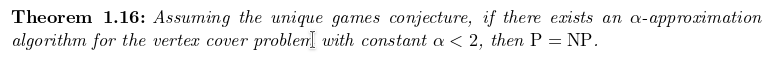
\includegraphics[width=1\textwidth]{images/vertexcover.png}
    \label{fig:mot1}
\end{figure}{}
\pause
\begin{figure}
    \centering
    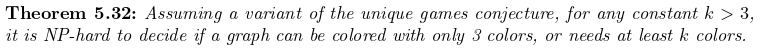
\includegraphics[width=1\textwidth]{images/coloring.png}
    \label{fig:mot2}
\end{figure}{}
\pause
\begin{figure}
    \centering
    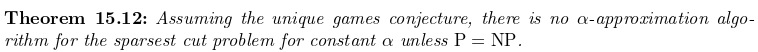
\includegraphics[width=1\textwidth]{images/sparsest.png}
    \label{fig:mot3}
\end{figure}{}
\pause
\begin{figure}
    \centering
    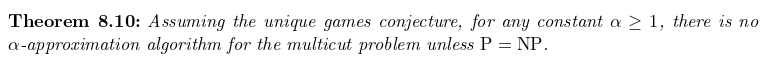
\includegraphics[width=1\textwidth]{images/multicut.png}
    \label{fig:multicut}
\end{figure}{}

\end{frame}

\begin{frame}
  \frametitle{Motivação}
\begin{figure}
    \centering
    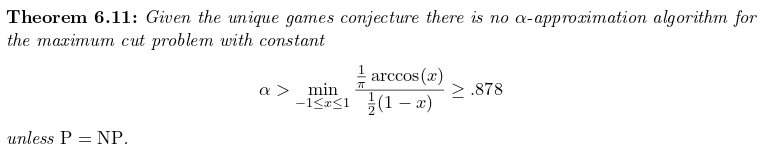
\includegraphics[width=1\textwidth]{images/maxcut.png}
    \label{fig:maxcut}
\end{figure}{}
\end{frame}

\begin{frame}[<+->]
  \frametitle{Motivação}

  \begin{itemize}
    \item Vimos anteriormente um algoritmo de aproximação para o problema Max-Cut.
    \begin{itemize}
        \item Utilizava Semidefinite Programming
        \item .878-aproximação, chamada de algoritmo de \emph{Goemans-Williamson}
    \end{itemize}
    \item Ao final da aula, foi visto um teorema: esse algoritmo é a melhor aproximação possível para o problema, assumindo a \emph{Unique Games Conjecture}.
    \item O que é a Unique Games Conjecture?
  \end{itemize}

\end{frame}

\begin{frame}
    \frametitle{Histórico}
    
    \begin{figure}
        \centering
        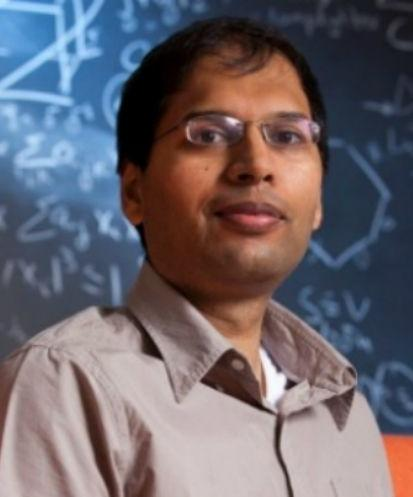
\includegraphics[width=0.5\textwidth]{images/subhash.jpg}
        \caption*{Subhash Khot}
    \end{figure}{}
    
\end{frame}

\begin{frame}
    \frametitle{Histórico}
    
    \begin{itemize}
        \item Coloração de grafos;
        \item Há diferença entre 3 cores e $k$ cores?
        \item Mais em \cite{history}.
    \end{itemize}
    
\end{frame}

\section{Unique Games e Unique Label Cover}

\begin{frame}[<+->]
    \frametitle{Unique Games}
    \begin{itemize}
        \item A \textbf{conjectura} do Unique Games é criada a partir do \textbf{problema} chamado Unique Games.
        \item O Unique Games é um problema de satisfação de restrições, ou seja, é uma versão específica do CSP (Constraint Satisfaction Problem).
    \end{itemize}
\end{frame}

\begin{frame}[<+->]
    \frametitle{Unique Games}
    \begin{itemize}
        \item O CSP é dado por:
        \begin{itemize}
            \item Entrada:
                \begin{itemize}
                    \item Universo $U$ de valores;
                    \item Variáveis $X_i \in U, \forall i \in \{1 \dots n\}$;
                    \item restrições $f:U^k \xrightarrow{} \{0,1\}$
                \end{itemize}
            \item Solução: Atribuição de um valor em $U$ para cada variável.
            \item Objetivo: maximizar o número de restrições satisfeitas.
        \end{itemize}
        \item Há a versão com pesos também.
        \item Exemplos de problemas CSP: MAX-CUT, MAX-SAT.
    \end{itemize}
\end{frame}

\begin{frame}[<+->]
    \frametitle{Unique Games}
    \begin{itemize}
        \item O Unique Games é um CSP \emph{binário}, ou seja, cada restrição corresponde a uma função em \emph{duas variáveis}.
        \item Além disso, para cada valor de $U$ de uma das variáveis da restrição, há \emph{exatamente um} valor para a outra variável que a satisfaz. Assim, uma restrição corresponde a uma função \emph{bijetora}.
    \end{itemize}
\end{frame}

\begin{frame}
    \frametitle{Unique Games Conjecture}
    \begin{conjectura}[Unique Games Conjecture: UGC]
        Dados quaisquer $\epsilon,\delta>0$, existe algum $k>0$ dependente de  $\epsilon$ e $\delta$, tal que para o problema Unique Games com universo de tamanho $k$, é \emph{\np-Difícil} distinguir entre instâncias nas quais pelo menos uma fração de $1-\epsilon$ das restrições pode ser satisfeita, e instâncias nas quais no máximo uma fração de $\delta$ das restrições pode ser satisfeita.
    \end{conjectura}
\end{frame}

\begin{frame}[<+->]
    \frametitle{Unique Games Conjecture}
    \begin{itemize}
        \item Informalmente, a UGC diz que é \np-Difícil diferenciar uma instância do problema na qual \emph{quase todas} as restrições são satisfeitas e uma em que \emph{quase nenhuma} é satisfeita.
        \item Um problema é chamado \emph{UG-Difícil} se ele é \np-Difícil considerando a UGC.
        \item Não se sabe se há algoritmo de aproximação para o Unique Games que garanta desempenho que refute a UGC.
    \end{itemize}
\end{frame}

\begin{frame}[<+->]
    \frametitle{Unique Label Cover}
    \begin{itemize}
        \item Como as restrições do Unique Games são funções de duas variáveis, é fácil perceber que há uma representação do problema como \emph{grafo}.
        \item A versão em grafo do problema possui um nome: \emph{Unique Label Cover}.
        \item Essa versão é tão comum, e mais fácil de entender, que em muitos lugares o Unique Games é apresentado diretamente com ela!
    \end{itemize}
\end{frame}

\begin{frame}[<+->]
    \frametitle{Unique Label Cover}
    \begin{itemize}
        \item Para a transformação do UG para o ULC, criamos \emph{permutações}.
        \begin{itemize}
            \item Uma permutação é um rearranjo do universo $U$ do problema que mapeia, para cada restrição, o valor de uma variável ao valor da outra tal que $f(X_i,X_j) = 1$.
            \item Isso pode ser feito pois a função é bijetora, e para universo de tamanho $k$, $U={1\dots k}$.
            \item Assim, podemos definir a permutação como $\pi(i) = j$ se $f(i,j) = 1$.
        \end{itemize}
    \end{itemize}
\end{frame}

\begin{frame}
    \frametitle{Transformação Unique Games-Unique Label Cover}
    Assim, a transformação é:
    \begin{block}{\Algoritmo{Transformação-UG-ULC}}
        \begin{algorithm}[H]
          Crie um grafo vazio não-direcionado $G=(V,E)$\;
          Para cada variável $X_u, u \in {1\dots n}$, insira o vértice $u$ em $V$\;
          \pause
          Para cada restrição $f(X_u,X_v)$, insira a aresta $(u,v)$ em E\;
          \pause
          Para toda aresta $(u,v)$, crie uma permutação $\pi_{uv}: U \xrightarrow{} U$ tal que $\pi_{uv}(i)=j$ se $f(i,j)=1$\;
          \pause
          Retorne $G, \pi$\;
        \end{algorithm}
    \end{block}
\end{frame}

\begin{frame}[<+->]
    \frametitle{Unique Label Cover}
    \begin{itemize}
        \item Assim, o problema se torna um de encontrar \emph{labels (rótulos)} em vértices tais que a maior quantidade de permutações são satisfeitas.
        \item Podemos verificar em tempo polinomial se \emph{todas} as arestas do grafo são satisfatíveis.
        \begin{itemize}
            \item Para toda componente conexa do grafo, teste todos os \textit{labels} para um vértice arbitrário.
            \item Para cada escolha, \emph{propague} para todos os outros, pelas permutações.
            \item Se todas as arestas são satisfatíveis, há algum \textit{label} que gera uma atribuição perfeita, e isso pode ser verificado em tempo polinomial, no pior caso.
        \end{itemize}
    \end{itemize}
\end{frame}

\begin{frame}[<+->]
    \frametitle{Unique Label Cover}
    \begin{itemize}
        \item Similarmente, saber se \emph{nenhuma} aresta é satisfatível também é trivial.
        \item Porém, o mesmo não pode ser dito para todos os outros casos.
        \item Pela UGC, se é desejado saber se uma \textbf{fração constante} de arestas é satisfatível, o problema é \np-Difícil para algum universo, independentemente da fração.   
        \end{itemize}
\end{frame}

\begin{frame}[<+->]
    \frametitle{Algoritmos para Unique Label Cover/Unique Games}
    \begin{itemize}
        \item Existe um algoritmo de aproximação de fator $1-\sqrt{\epsilon \log n}$ para o Unique Games/Unique Label Cover, baseado em \emph{Semidefinite Programming}. 
        \begin{itemize}
            \item Esse algoritmo funciona para instâncias nas quais uma fração de $1-\epsilon$ das arestas/restrições são satisfatíveis.
            \item Se $\epsilon \in O(1/\log n)$, essa aproximação é constante.
            \item Não iremos mostrar esse algoritmo hoje, mas está especificado e demonstrado em \cite{design_approx_algs}.
        \end{itemize}
        \item Há também algoritmos \emph{subexponenciais} para o problema e outros relacionados, ao contrário de diversos outros problemas \np-Difíceis. Alguns podem ser vistos em \cite{subexponential}.
    \end{itemize}
\end{frame}{}

\section{Consequências da UGC}

\begin{frame}
    \frametitle{Problemas Relacionados à UGC}
    \begin{figure}
        \centering
        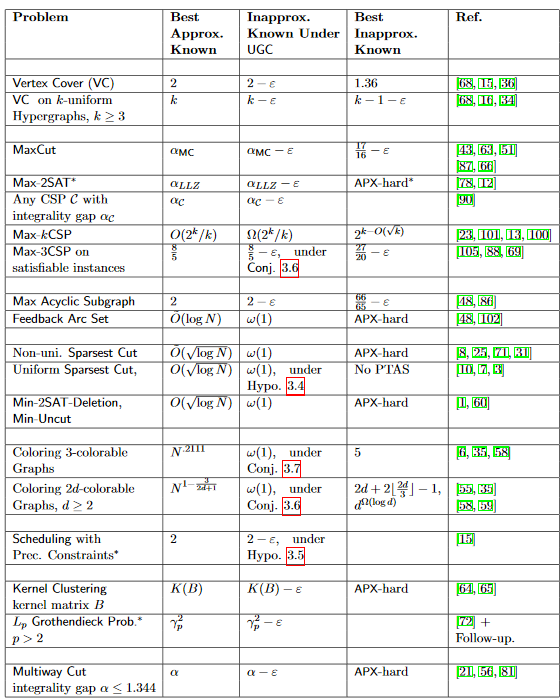
\includegraphics[width=0.55\textwidth]{images/reducoes.png}
        \caption{Reduções obtidas a partir da UGC.}
        \label{fig:reducoes}
    \end{figure}
\end{frame}{}

\begin{frame}[<+->]
    \frametitle{Consequências da UGC}
    \begin{itemize}
        \item Desde 2002, a UGC teve diversas aplicações em problemas relacionados.
        \item A figura \ref{fig:reducoes} foi extraída de \cite{survey}, que também possui diversos desenvolvimentos e conclusões em cima da UGC.
        \item Como visto na figura, o principal uso da UGC foi para provas de \emph{inaproximabilidade}, muitas vezes junto com outra técnica, como PCP.
        \item Ela também deu origem a diversas \emph{variantes}.
        \item Deste ponto em diante, veremos duas reduções para problemas que provam inaproximabilidade ou que uma aproximação conhecida é a melhor possível.
    \end{itemize}
\end{frame}{}

\section{Redução para Multicut}
\begin{frame}[<+->]
    \frametitle{Multicorte}
        \begin{itemize}
            \item Relembrando o problema do multicorte:
                \begin{itemize}
                    \item Entrada:
                        \begin{itemize}
                            \item grafo G=(V,E);
                            \item custo das arestas $c_e \ge 0,\, e \in E$;
                            \item pares de vértices fonte-ralo $s_1-t_1, \dots, s_k-t_k,\,s,t \in V$.
                        \end{itemize}
                    \item Solução: conjunto de arestas $F$ nas quais ao serem removidas desconectam todos os pares $s_1-t_1, \dots, s_k-t_k$.
                    \item Objetivo: minimizar o custo total das arestas F removidas.
                \end{itemize}
        \end{itemize}        
\end{frame}{}

\begin{frame}
    \frametitle{Exemplo de Multicorte}
    
    \begin{figure}
        \centering
        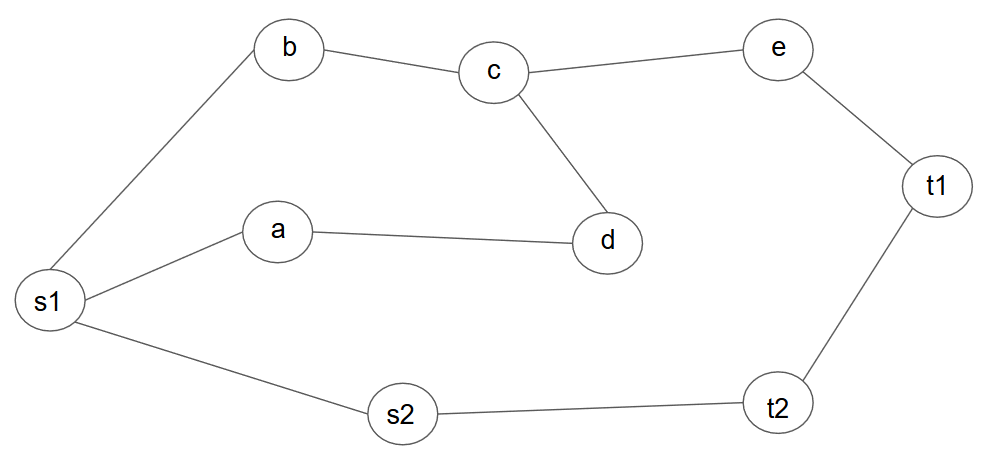
\includegraphics[width=1\textwidth]{images/multicutExample.png}
        %\caption*{Subhash Khot}
    \end{figure}{}
    
\end{frame}

\begin{frame}
    \frametitle{Exemplo de Multicorte}
    
    \begin{figure}
        \centering
        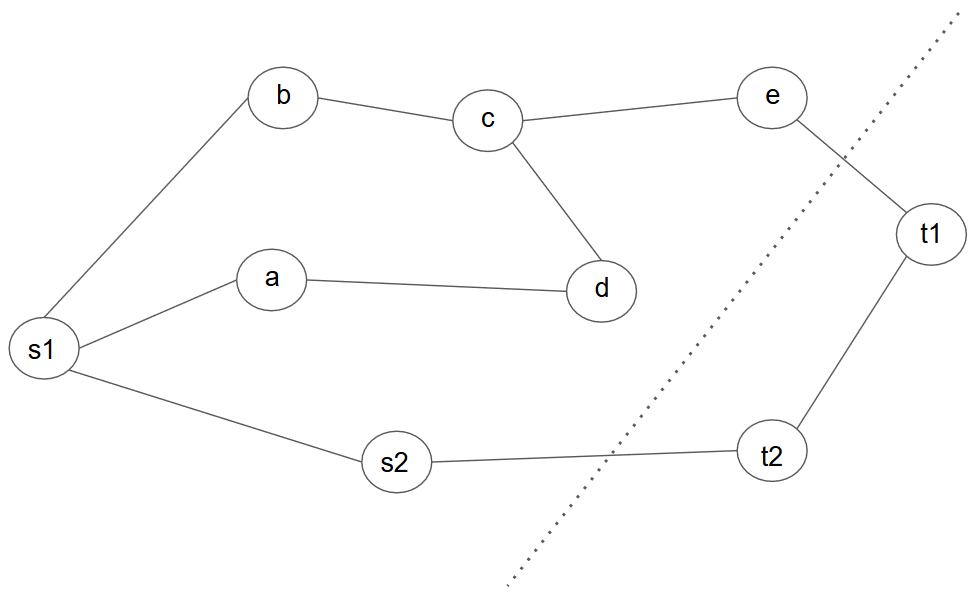
\includegraphics[width=1\textwidth]{images/multicutEdges.png}
        %\caption*{Subhash Khot}
    \end{figure}{}
    
\end{frame}

\begin{frame}
    \frametitle{Exemplo de Multicorte}
    
    \begin{figure}
        \centering
        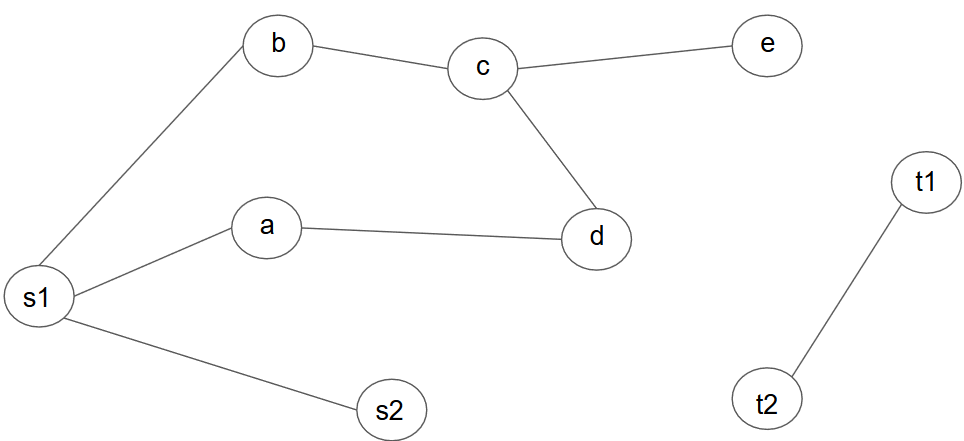
\includegraphics[width=1\textwidth]{images/multicutSol.png}
        %\caption*{Subhash Khot}
    \end{figure}{}
    
\end{frame}

\begin{frame}[<+->]
    \frametitle{Redução para Multicorte}
       \begin{teorema}[1] \label{multicut}
        Assumindo a conjectura do Unique Games, para qualquer constante $\alpha \ge 1$, não existe $\alpha$-aproximação para o problema do multicorte a não ser que $\pp = \np$.
        \end{teorema}
        \begin{itemize}
            \item Pelo teorema, é \emph{UG-Difícil} aproximar o problema do multicorte por qualquer constante maior ou igual a 1.
            
            \item Para a redução da UG para multicorte utilizamos um caso especial da UG chamada MAX 2LIN(k).
        \end{itemize}
\end{frame}{}

\begin{frame}[<+->]
    \frametitle{Redução para Multicorte}
        MAX 2LIN(k):
        \begin{itemize}
            \item Entrada:
            \begin{itemize}
                \item L={0,...,k-1}, $k \in \mathbb{Z}$;
                \item Variáveis (vértices) $\in V$;
                \item Restrições (arestas) $\in E$;
                \item $\forall uv \in E$, temos $c_{uv} \in L$ tal que $\pi_{uv}(i)=i-c_{uv}(mod\,k)$, ou seja, $uv$ é satisfeita $\iff$ os vértices $u$ e $v$ recebem rótulos $i,j$ tais que $i-j=c_{uv}(mod\,k)$;
              \end{itemize}
            \item Solução: Atribuição de rótulos R, tal que  $\forall u \in V$, existe um rótulo $r_u \in L$;
            \item Objetivo: Maximizar número de arestas $uv \in E$ satisfeitas.
        \end{itemize}
\end{frame}{}

\begin{frame}
    \frametitle{Redução para Multicorte}
        \begin{conjectura}[Linear Unique Games Conjecture: LUGC]
            Dados quaisquer $\epsilon,\delta>0$, existe algum $k>0$ dependente de  $\epsilon$ e $\delta$, a versão do unique games MAX 2LIN(k) com L={0,...,k-1}, é \emph{\np-Difícil} distinguir entre instâncias nas quais pelo menos uma fração de $1-\epsilon$ das arestas pode ser satisfeita, e instâncias nas quais no máximo uma fração de $\delta$ das arestas pode ser satisfeita.
        \end{conjectura}    
\end{frame}{}

\begin{frame}[<+->]
    \frametitle{Redução para Multicorte}
         Para provar o \emph{Teorema \ref{multicut}} são necessários 2 lemas:
        \begin{lema}[1] \label{lema1multicut}
            Para qualquer $\epsilon$ tal que $0 \le \epsilon \le 1$, dado uma solução viável de uma instância de  MAX 2LIN(k) que satisfaz pelo menos $(1-\epsilon)|\,E\,|$ arestas, então existe uma solução viável para uma instância do multicut com custo de no máximo $\epsilon|\,E'\,|$.
        \end{lema}
\end{frame}{}

\begin{frame}[<+->]
    \frametitle{Redução para Multicorte}
        Prova do Lema \ref{lema1multicut}:
        %reduzir MAX2 LIN(k) para multicorte:
        \begin{itemize}
          \item Seja I uma instância do MAX 2LIN(k) com grafo $G=(V,E)$, universo $L$ de rótulos de tamanho $k$ e $C$ o conjunto de pesos das arestas de $E$;
          \item Faça uma instância I' do multicorte da seguinte maneira: 
          \begin{itemize}
            \item G'=(V',E') com V' = V x L;
            \item Arestas em E' entre pares vértice-rótulo (u,i) e (v,j) $\iff uv \in E$ e $i-j=c_{uv}(mod\,k)$;
            \item Também faça os pares fontes-ralo serem s=(u,i) e t=(u,j) para todo u $\in V$ e $i \ne j$;
          \end{itemize}
          \item Note que $E'=k|\,E\,|$ e $V'=k|\,V\,|$;
          \end{itemize}
\end{frame}{}

\begin{frame}
    \frametitle{Redução para Multicorte}
    
    \begin{figure}
        \centering
        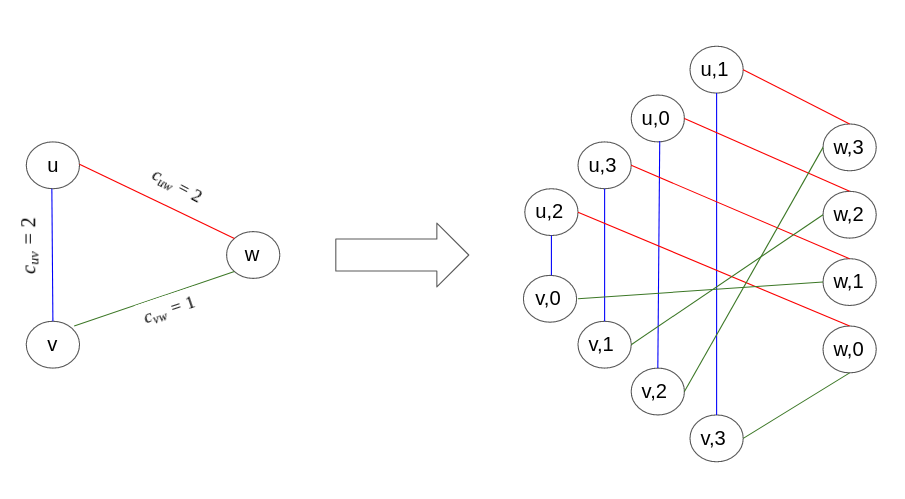
\includegraphics[width=1\textwidth]{images/graphGline.png}
        %\caption*{Subhash Khot}
    \end{figure}{}
    
\end{frame}

\begin{frame}[<+->]
    \frametitle{Redução para Multicorte}
        Solução do multicorte:
        \begin{itemize}
            \item Suponha uma rotulação $x_u \in L$ de G que satisfaz pelo menos $(1-\epsilon)|\,E\,|$ arestas de G;
            \item Particione V' em k partes, $V'_0,\dots,V'_{k-1}$, onde $V'_c=\{(u,x_u+c(mod\,k))\} \forall u \in V$, ou seja, a c-ésima parte será o conjunto de vértices cuja rotulação satisfazem uma aresta de custo c;          \item Note que s=(u,i) e t=(u,j) $\forall u\in V$ e $i \ne j$; estão em diferentes partes da partição, portanto, ao remover todas arestas com extremos em diferentes partes da partição obtemos uma solução do multicorte;
        \end{itemize}
\end{frame}{}

\begin{frame}
    \frametitle{Redução para Multicorte}
    
    \begin{figure}
        \centering
        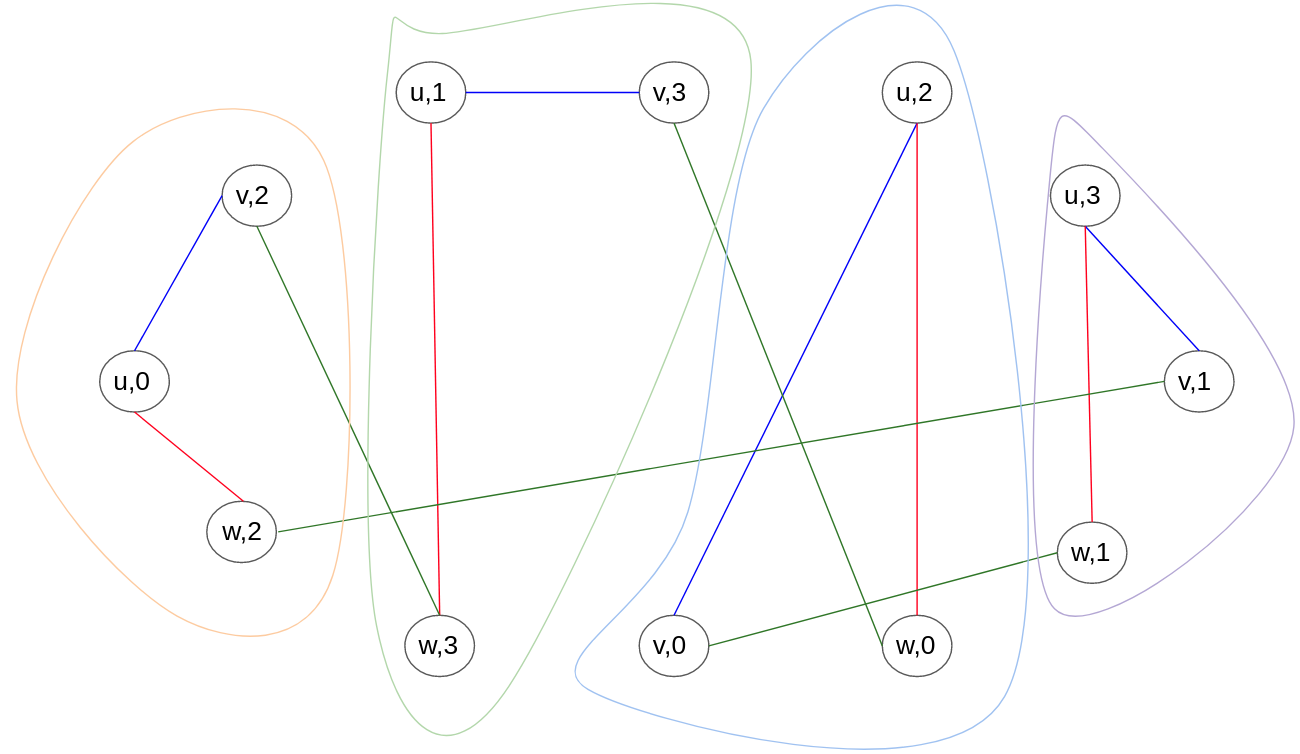
\includegraphics[width=1\textwidth]{images/Partition.png}
        %\caption*{Subhash Khot}
    \end{figure}{}
    
\end{frame}

\begin{frame}
    \frametitle{Redução para Multicorte}
    
    \begin{figure}
        \centering
        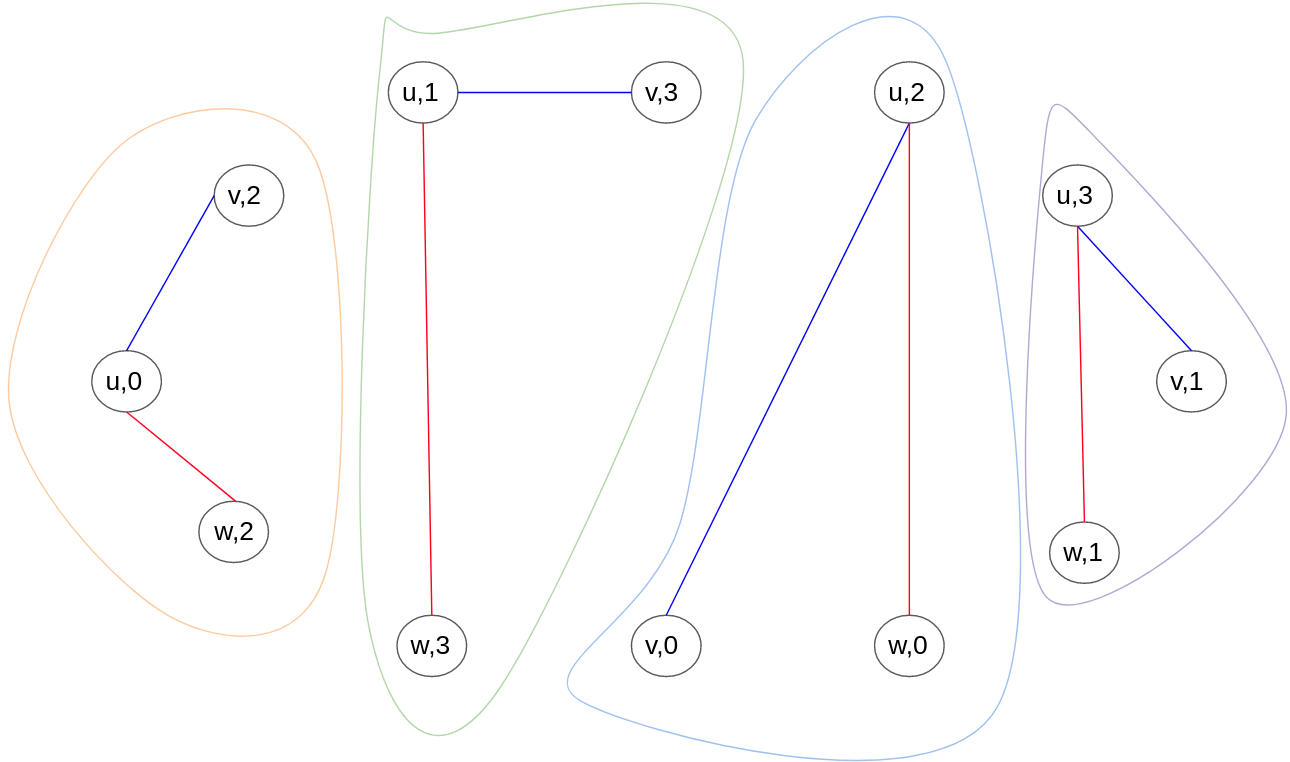
\includegraphics[width=1\textwidth]{images/RemovedEdges.png}
        %\caption*{Subhash Khot}
    \end{figure}{}
    
\end{frame}

\begin{frame}[<+->]
    \frametitle{Redução para Multicorte}
        Custo dessa solução:
        \begin{itemize}
            \item Considere qualquer aresta $((u,i),(v,j)) \in E’$ tal que (u,i) e (v,j) estão em diferentes partes da partição. Demonstraremos que a aresta (u,v) no grafo original não é satisfeita pelo rotulamento dado;
            \item Pela construção de E’ sabemos que $i-j=c_{uv}(mod\,k)$. Também sabemos que (u,i) e (v,j) estão em diferentes partes da partição;
            \item Suponha que $(u,i) \in V_c$ e $(v,j) \in V_c$' para $c \ne c'$. Então $i=x_u+c(mod\,k)$ e $j=x_v+c'(mod\,k)$, e portanto:
        \end{itemize}
\end{frame}{}

\begin{frame}[<+->]
    \frametitle{Redução para Multicorte}
        \begin{itemize}
            \item Suponha que $(u,i) \in V_c$ e $(v,j) \in V_c$' para $c \ne c'$. Então $i=x_u+c(mod\,k)$ e $j=x_v+c'(mod\,k)$, e portanto:
            \begin{align*}
                c_{uv} &= i-j(mod\,k) \\
                       &= (x_u+c)-(x_v+c')(mod\,k) \\
                       &= (x_u-x_v)+(c+c')(mod\,k) \\
                       &\ne x_u-x_v(mod\,k)
            \end{align*}
            pois $c \ne c'$;
            \item Como uma aresta é satisfeita $\iff c_{uv} = i-j(mod\,k)$, isto significa que arestas entre vértices de diferentes partições não são satisfeitas. Como no máximo $\epsilon|\,E\,|$ arestas não são satisfeitas em MAX 2LIN(k), no máximo $\epsilon k|\,E\,| = \epsilon|\,E'\,|$ arestas são removidas no multicorte.
        \end{itemize}
\end{frame}{}

\begin{frame}[<+->]
    \frametitle{Redução para Multicorte}
     \begin{lema}[2] \label{lema2multicut}
        Para qualquer $\epsilon$ tal que $0 \le \epsilon \le 1$, dado uma solução de uma instância do multicorte de custo máximo $\epsilon|\,E'\,|$, então existe uma solução para uma instância do MAX 2LIN(k) que satisfaz pelo menos (1-2$\epsilon$)$|\,E\,|$ arestas.
    \end{lema}
    Prova do Lema \ref{lema2multicut} omitida por simplificação, mas é o caminho inverso da prova do Lema \ref{lema1multicut}. Pode ser vista em \cite{design_approx_algs}.
\end{frame}{}

\begin{frame}[<+->]
    \frametitle{Redução para Multicorte}
    Prova do Teorema \ref{multicut}:
    \begin{itemize}
        \item Suponha que existe $\alpha$-aproximação para o problema do multicorte;
        \item Então utilizando este algoritmo e o Lema \ref{lema1multicut}, sabemos que: dado uma instância do MAX LIN2(k), na qual pelo menos (1-$\epsilon$)$|\,E\,|$ arestas são satisfeitas, podemos encontrar uma solução do multicorte de custo $\epsilon \alpha|\,E'\,|$;
        \item Pelo Lema \ref{lema2multicut} sabemos obter uma solução do MAX 2LIN(k), a partir deste multicorte, na qual pelo menos (1-2$\epsilon \alpha$)$|\,E\,|$ arestas satisfeitas;
    \end{itemize}
\end{frame}{}

\begin{frame}[<+->]
    \frametitle{Redução para Multicorte}
    Prova do Teorema \ref{multicut}:
    \begin{itemize}
        \item Se a instância do MAX LIN2(k) satisfaz no máximo $\delta|\,E\,|$ arestas, então este algoritmo satisfaz no máximo $\delta|\,E\,|$ arestas;
        \item Fazendo $\epsilon < \frac{1-\delta}{2\alpha}$, então temos que $(1-2\epsilon\alpha)|\,E\,| > \delta|\,E\,|$.
        \item Isto implica que nosso algoritmo consegue distinguir entre instâncias nas quais pelo menos (1-$\epsilon$)$|\,E\,|$ arestas são satisfeitas e instâncias nas quais no máximo $\delta|\,E\,|$ arestas são satisfeitas;
        \item Dado a UG, isto implica que $\pp = \np$. $\square$
    \end{itemize}
\end{frame}{}


%%%%%%%%%%%%%%%%%%%%%%%%%%%%%%%%%%%%%%%%%%%%%%%%%%%%%%%%%%%%%%%%%%%%%%%%%%%%%%%%%%%%%%%%%%%%%%%%%%%%%%%%%%%%%%%%%%%%%%%%%%%%%%%%%%%%%%%%%%%%%%%%%%


\section{Redução para Max-Cut}

\begin{frame}[<+->]
    \frametitle{O problema Max-Cut}
        \begin{itemize}
            \item Relembrando o problema do Max-Cut:
                \begin{itemize}
                    \item Entrada:
                        \begin{itemize}
                            \item grafo $G=(V,E)$ não-direcionado;
                        \end{itemize}
                    \item Solução:
                        \begin{itemize}
                            \item Partição de vértices $V_1$ e $V_2$:
                            % \item $V_1 \cup V_2 = V$ \& $V_1 \cap V_2 = \oslash$
                        \end{itemize}
                    \item Objetivo:
                        \begin{itemize}
                            \item Maximizar o número de arestas no corte
                            \item $\forall e\in E$, temos que $e $ está no corte se: $e=(u,v)|u\in V_1 \ \& \ v\in V_2 $
                        \end{itemize} 
                \end{itemize}
        \end{itemize}        
\end{frame}{}


\begin{frame}[<+->]
    \frametitle{Inaproximibilidade do Max-Cut}
        \begin{teorema}
            Assumindo a conjectura do Unique Games, não existe $\alpha$-aproximação para o problema do corte máximo com constante
            \[\alpha > \min_{-1 \le x \le 1} \frac{\frac{1}{\pi} \arccos{x}}{\frac{1}{2}(1-x)} \ge .878 \]
            a não ser que $\pp = \np$.
        \end{teorema}
        \begin{itemize}
            \item Pelo teorema, é \emph{UG-Difícil} aproximar o problema do Max-Cut por qualquer constante $\alpha$ maior que $.878$.
            \item Para a redução da UG para Max-Cut, utilizamos uma variação equivalente da UGC denominada \textit{Bipartite Unique Games Conjecture}.
        \end{itemize}
\end{frame}{}


\begin{frame}[<+->]
    \frametitle{Inaproximibilidade do Max-Cut}
        \begin{conjectura}[BUGC]
        Dados \mage{quaisquer $\epsilon,\delta>0$}, existe algum $k>0$ dependente de $\epsilon$ e $\delta$, tal que para o problema Unique Games com universo de tamanho $k$ em \mage{grafos bipartidos nos quais todos os vértices de uma partição têm o mesmo grau}, é \np-Difícil distinguir entre instâncias nas quais pelo menos uma fração de $1-\epsilon$ das restrições pode ser satisfeita, e instâncias nas quais no máximo uma fração de $\delta$ das restrições pode ser satisfeita.
        \end{conjectura}
        \begin{itemize}
            \item A probabilidade selecionar uma aresta aleatória $(\red{v},\green{u})$ dado um vértice $\red{v}$, é a mesma para qualquer aresta
            \item Dado $\red{v}$, podemos sortear uma segunda aresta $(\red{v},\blue{w})$, resultando em duas arestas que compartilham $\red{v}$
            \item seleção \mage{aleatória} e \mage{uniforme}
            \item podemos selecionar \mage{$\epsilon$ arbitariamente pequeno}
        \end{itemize}
\end{frame}{}

\begin{frame}[<+->]
\frametitle{Relembrando PCP}
    \begin{itemize}
        % \item \textbf{Classe NP:} Problemas de decisão que, dado uma instância SIM e uma prova, podemos verificar a validade da prova em tempo polinomial. (EX: Sudoku)
        \item \textbf{Verificador PCP:} Recebe uma \red{instância $x$} de um problema NP e uma \red{prova $\pi$}. Lendo $r$ bits aleatórios, \red{acessa apenas $q$} bits da prova.
        \begin{itemize}
            \item \textbf{Completeness:} Para uma instância \green{SIM}, há uma prova com probabilidade de \green{aceite de pelo menos \textit{c}}
            \item \textbf{Soundness:} Para uma instância NÃO, qualquer prova tem probabilidade de aceite de no máximo \textit{s} 
        \end{itemize}
        \item \textbf{CSPs:} Verificadores PCP são \red{geram CSPs} onde os bits acessados são as variáveis e os testes entre eles, restrições.
    \end{itemize}

\end{frame}{}


\begin{frame}[<+->]
\frametitle{PCP e Max-Cut}
    \begin{lema}
        Supondo a BUGC, para qualquer constante positiva $\gamma>0$ e qualquer $\rho \in (-1,0)$, \textcolor{red}{$\np \subseteq PCP(\log (n),2)$}, onde o verificador tem \red{\textit{completeness} no mínimo $\frac{1}{2} (1-\rho)-\gamma$} e \textit{soundness} no máximo $\frac{1}{\pi} \arccos{\rho} + \gamma$ e o verificador \red{aceita apenas se dois bits são diferente}.
    \end{lema}
    \begin{itemize}
        % \item \textbf{Teorema PCP:} $\np \subseteq PCP[\log n,1]$
        \item \textbf{Se o Lema é verdade, o Teorema também é?}
        \item Em outras palavras: \\ 
            O verificador gera um \red{CSP equivalente ao Max-Cut}?
    \end{itemize}
\end{frame}{}

\begin{frame}[<+->]
\frametitle{CSP e Max-Cut}
    \begin{itemize}
        \item Dada uma instância de $\Pi \in$ NP-Completo codificada para o PCP mencionado
        \item Suponha que os bits da prova sejam vértices:
        \begin{itemize}
            \item Se o bit for 1, $v\in V_1$
            \item Se o bit for 0, $v\in V_2$
        \end{itemize}
        \item Para todo possível par de bits $(u,v)$ comparados, cria-se uma aresta $(u,v)$ tal que $e\in E$
        \item Se os bits $(u,v)$ forem diferentes, $(u,v)$ está no corte.
        \item Geramos um resultado $G(V_1,V_2,E)$ do Max-Cut.
    \end{itemize}
\end{frame}{}

\begin{frame}[<+->]
\frametitle{CSP e Max-Cut}
    \begin{itemize}
        \item Suponha \red{$P\ne NP$}
        \item Temos \red{$|E|=Z_{UB}$ restrições} (número de arestas). 
        \item Temos que $Opt$ é o número restrições satisfeitas (corte).
        \item Suponha que há $\alpha$-aproximação para o Max-Cut tal que \red{$\alpha > \frac{s}{c}$}
        \item podemos encontrar um \red{valor aproximado $X$} em tempo polinomial tal que \red{$Opt \geq X > \frac{s}{c} \cdot Opt$}
        \item Mas pelo teorema PCP:
        \begin{itemize}
            \item \textcolor{red}{SIM} $\leftrightarrow Opt \geq c \cdot Z_{UB} \leftrightarrow  Opt \geq \textcolor{red}{X > s \cdot Z_{UB}}$
            \item \textcolor{red}{NÃO} $\leftrightarrow Opt \leq s \cdot Z_{UB} \leftrightarrow \textcolor{red}{s \cdot Z_{UB} \geq X} > \frac{s}{c} \cdot Opt$
        \end{itemize}
        \item Logo, podemos resolver em tempo polinomial um problema NP-Completo
        \item \textbf{Contradição:} Não há $\alpha$-app. a não ser que $P=NP$
    \end{itemize}
\end{frame}{}

\begin{frame}[<+->]
\frametitle{CSP e Max-Cut}
    \begin{figure}
            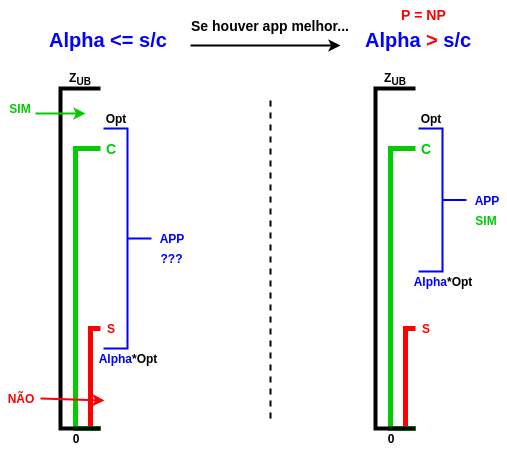
\includegraphics[width=0.8\textwidth]{images/gap.png}
    \end{figure}{}
\end{frame}{}

\begin{frame}[<+->]
\frametitle{CSP e Max-Cut}
    \begin{itemize}
        \item \textbf{Se o Lema é verdade, o Teorema também é?} \textcolor{pine}{\textbf{SIM}}
        \item Mas \red{como construir o PCP} descrito pelo Lema?
        \item Se a conjetura BUGC for verdadeira, isso é possível!
        \item \textbf{Parte difícil:} Codificar uma instância da BUGC em um PCP e provar que lendo apenas 2 bits:
        \begin{itemize}
            \item Há uma prova para \green{caso SIM aceita com probabilidade $\geq c$}
            \item Toda prova caso NÃO é aceita com probabilidade $\leq s$
        \end{itemize}
        \item \red{Lembrando: $c \geq \frac{1}{2}(1-\rho)$ }
    \end{itemize}
\end{frame}{}

\begin{frame}[<+->]
\frametitle{Conceitos necessários}
    \begin{itemize}
        \item \textbf{Funções ditadoras:} $f:\{0,1\}^k \xrightarrow\ \{0,1\}$, tal que para $f(x_1,...,\red{x_i},...,x_k)=\red{x_i} $ para algum $\red{i}\in [\org{0},\org{k}]$ \\
    \end{itemize}
    \begin{figure}
            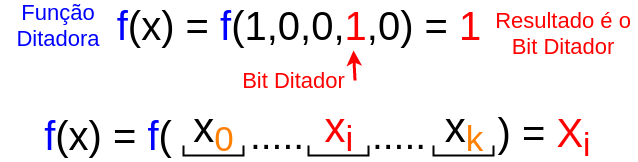
\includegraphics[width=1\textwidth]{images/dictators.png}
    \end{figure}{}
\end{frame}{}

\begin{frame}[<+->]
\frametitle{Codificando a prova}
    \begin{itemize}
        \item Suponha 2 rótulos possíveis: $L=\{1,2\}\ \& \ |L|=k=2$
        \item Dado a prova:  \textcolor{red}{$v=1$}, \textcolor{pine}{$u=2$} e \textcolor{blue}{$w=1$} (Vértice=Rótulo)
        \item Temos as funções ditadoras: $x\in \{0,1\}^k, \ f_{\red{v}}(x_{\red{1}},-)=x_{\red{1}}, \ f_{\green{u}}(-,x_{\green{2}})=x_{\green{2}}, \ f_{\textcolor{blue}{w}}(x_{\textcolor{blue}{1}},-)=x_{\textcolor{blue}{1}}$
        % \item Transformando em uma cadeia de bits: 
        %     \begin{itemize}
        %     \item $ [f_{\red{v}}(\red{0},0), f_{\red{v}}(\red{0},1), f_{\red{v}}(\red{1},0), f_{\red{v}}(\red{1},1)] \ \ =  \red{[0,0,1,1]}$
        %     \item $ [f_{\green{u}}(0,\green{0}), f_{\green{u}}(0,\green{1}), f_{\green{u}}(1,\green{0}), f_{\green{u}}(1,\green{1})] \ \ = \green{[0,1,0,1]}$
        %     \item $ [f_{\blue{w}}(\blue{0},0), f_{\blue{w}}(\blue{0},1), f_{\blue{w}}(\blue{1},0), f_{\blue{w}}(\blue{1},1)] = \blue{[0,0,1,1]}$
        %     \end{itemize}
        \end{itemize}
        \begin{figure}
                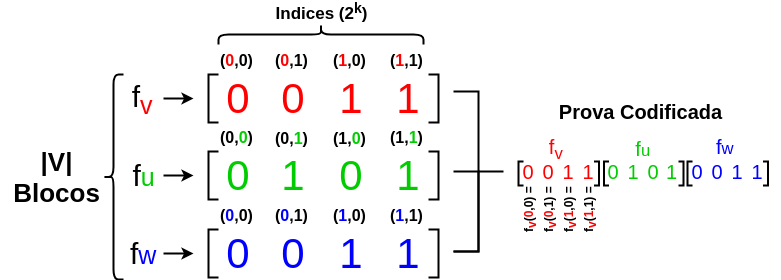
\includegraphics[width=1\textwidth]{images/encoding.png}
        \end{figure}
        \begin{itemize}
        \item Prova codificada: \ $\red{[0,0,1,1]} \green{[0,1,0,1]} \blue{[0,0,1,1]} $ (bit vector)
        \item Tamanho: $\red{2^k}\cdot \green{2^k}\cdot \blue{2^k} = |V|\cdot 2^k$ (\textit{long Code})
    \end{itemize}
\end{frame}{}

\begin{frame}[<+->]
\frametitle{Conceitos necessários}
    \begin{itemize}
        \item \textbf{Ruído:} Dado $x\in \{0,1\}^k$, podemos criar \blue{$y$} invertendo independentemente cada bit de $x$ com probabilidadade \red{$\frac{1}{2} (1-\rho)$}. Denota-se esse processo por $y\sim_\rho x$
    \end{itemize}
    \begin{figure}
            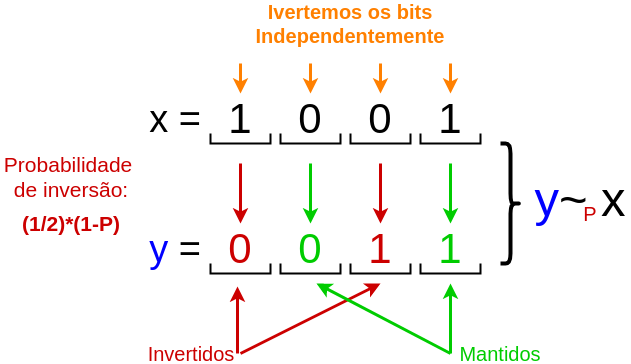
\includegraphics[height=0.4\textwidth]{images/noise.png}
    \end{figure}
    \begin{itemize}
        \item \textbf{OBS:} Probabilidade de alterar o resultado de uma função ditadora é a \red{probabilidade de inversão do bit ditador}
    \end{itemize}
\end{frame}{}

\begin{frame}[<+->]
\frametitle{Conceitos necessários}
    \begin{itemize}
    \item \textbf{Permutação de bits -} Suponha tal permutação:
    \begin{figure}
        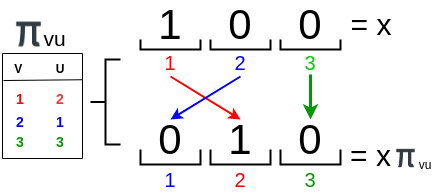
\includegraphics[height=0.3\textwidth]{images/bit_perm.png}
    \end{figure}{}
    \end{itemize}
\end{frame}{}

\begin{frame}[<+->]
\frametitle{Conceitos necessários}
    \begin{itemize}
    \item Note que dada uma aresta $(\red{v},\blue{u})\in E$ tal que $\red{v}$ tem rótulo $\red{i}$ e que  $\blue{u}$ tem rótulo $\blue{j}$, e dado um $x\in \{0,1\}^k$ qualquer, temos:\\
    \textbf{***}  $ \pi_{\red{v}\blue{u}}(\red{i}) = \blue{j} \xrightarrow{} f_{\red{v}}(x)=f_{\blue{u}}(x\circ \pi_{\red{v}\blue{u}})$\\ uma vez que o $\red{i}$-ésimo bit de $x$ é levado para o $\blue{j}$-ésimo bit de $x\circ \pi_{\red{v}\blue{u}}$ pela permutação
    \end{itemize}
    \begin{figure}
        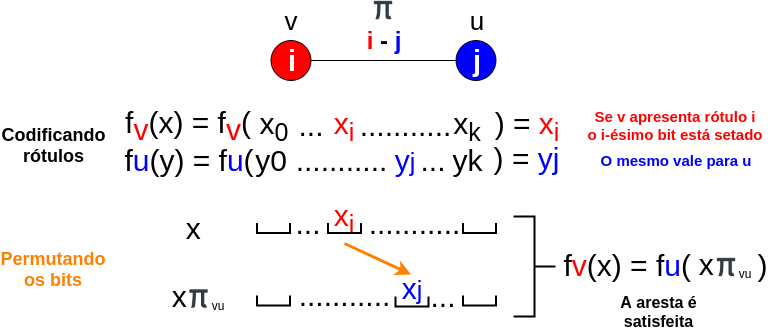
\includegraphics[width=1\textwidth]{images/satisfied.png}
    \end{figure}{}
\end{frame}{}

\begin{frame}[<+->]
\frametitle{O verificador PCP}
    \begin{itemize}
        \item Paramêtros: 
        \begin{itemize}
            \item $G(V_1, V_2, E)$ - Instância do BUGC
            \item $\pi$ - Prova codificada
    \end{itemize}
    \item \textbf{Algoritmo:}
    \begin{itemize}
        \item Seleciona um vértice $v\in V_1$
        \item Seleciona um vizinho de $v$, $u\in V_2$
        \item Seleciona outro vizinho de $v$, $w\in V_2$
        \item Sorteia uma \textit{string} $x\in \{0,1\}^k$
        \item Calcula $x\circ \pi_{vu}$ 
        \item Calcula $y\sim_\rho x$
        \item Calcula $y\circ \pi_{vw}$
        \item \textbf{Query:} $b_u \leftarrow{} f_u(x\circ \pi_{vu})$; $b_w \leftarrow{} f_w(y\circ \pi_{vw})$
        \item Se \green{$b_u \ne b_w$}, retorna \green{SIM}, caso contrário, NÃO.
    \end{itemize}
    \item \textbf{Se \green{$G(V_1,V_2,E)$} tem pelo menos \green{$\geq 1-\epsilon$} das arestas satisfatíveis, qual a probabilidade de \green{SIM}?}
    \item \red{\textbf{Lembrando:} Precisa ser $\geq \frac{1}{2}(1-\rho)$ (\textit{completeness})}
    \end{itemize}
\end{frame}{}

\begin{frame}[<+->]
\frametitle{O verificador PCP}
    \begin{itemize}
    \item \textbf{Duas arestas aleatórias:}
    \begin{itemize}
        \item Seleciona um vértice $\red{v}\in V_1$
        \item Seleciona um vizinho de $\red{v}$, $\green{u}\in V_2$
        \item Seleciona outro vizinho de $\red{v}$, $\blue{w}\in V_2$
    \end{itemize}
    \item Todo vértice $\red{v}\in V_1$ tem mesmo grau (BUGC)
    \item $(\red{v},\green{u})$ e $(\red{v},\blue{w})$ - aleatoriedade e uniformidade
    \item Probabilidade de uma aresta ser satisfeita: $\geq  (1-\epsilon)$
    \item Então, a probabilidade de $(\red{v},\green{u})$ e $(\red{v},\blue{w})$ serem satisfeitas é: \\ $\mage{(1-2\cdot\epsilon)} \leq (1-2\epsilon + \epsilon^2) = (1-\epsilon)^2$
    \end{itemize}
\end{frame}{}


\begin{frame}[<+->]
\frametitle{O verificador PCP}
    \begin{itemize}
    \item \textbf{Inserção de ruído:}
    \begin{itemize}
        \item Calcula $\brown{y}\sim_\rho x$
        \item Calcula $\brown{y}\circ \pi_{\red{v}\blue{w}}$
    \end{itemize}
    \item Qual a probabilidade de que $f_{\blue{w}}(\brown{y}\circ \pi_{\red{v}\blue{w}}) \ne f_{\blue{w}}(x\circ \pi_{\red{v}\blue{w}})$?
    \item Probabilidade de \textbf{inversão do bit ditador}: \mage{$\frac{1}{2}(1-\rho)$}
    \end{itemize}
\end{frame}{}

\begin{frame}[<+->]
\frametitle{O verificador PCP}
    \begin{itemize}
    \item \textbf{Acessando a prova:} 
        \begin{itemize}
            \item \textbf{Query:} $b_u \leftarrow{} \red{f_u(}\blue{x\circ \pi_{vu}}\red{)}$; $b_w\leftarrow{} \red{f_w(}\blue{y\circ \pi_{vw}}\red{)}$
        \end{itemize}
        \item $\red{f_u()}$ e $\red{f_w()}$ são os \red{blocos} codificados
        \item $\blue{x\circ \pi_{vu}}$ e $\blue{y\circ \pi_{vw}}$ são \blue{índices} dos \red{blocos}
        \item $f_u(x\circ \pi_{vu})$ e $ f_w(y\circ \pi_{vw})$ representam \mage{2 bits}
    \end{itemize}
\end{frame}{}

\begin{frame}[<+->]
\frametitle{O verificador PCP}
    \begin{itemize}
    \item \textbf{Comparando bits:} 
        \begin{itemize}
            \item Se \green{$b_u \ne b_w$}, retorna \green{SIM}, caso contrário, NÃO.
        \end{itemize}
        \item \textbf{Probabilidade de que \green{$f_u(x\circ \pi_{vu}) \ne f_w(y\circ \pi_{vw})$}?}
        \item Se $(\red{v},\green{u})$ satisfeita, $f_{\red{v}}(x) = f_{\green{u}}(x\circ \pi_{\red{v}\green{u}}) \xrightarrow{}$ \mage{$(1- \epsilon)$}
        \item Se $(\red{v},\blue{w})$ satisfeita, $f_{\red{v}}(x) = f_{\blue{w}}(x\circ \pi_{\red{v}\blue{w}}) \xrightarrow{}$ \mage{$(1- \epsilon)$}
        \item $f_{\green{u}}(x\circ \pi_{\red{v}\green{u}}) = f_{\blue{w}}(x\circ \pi_{\red{v}\blue{w}}) \xrightarrow{}$ \mage{$\geq(1-2\cdot \epsilon)$}
        \item $f_{\blue{w}}(x\circ \pi_{\red{v}\blue{w}}) \ne f_{\blue{w}}(\brown{y}\circ \pi_{\red{v}\blue{w}}) \xrightarrow{}$ \mage{$\frac{1}{2}(1-\rho)$}
        \item Probabilidade de ambas satisfeitas e inverteida com ruído?\\
        $\geq (1-2\cdot \epsilon)\cdot \frac{1}{2}(1-\rho)$
        \item Podemos escolher \mage{$\epsilon$ arbritariamente pequeno}:\\
        \red{$\geq \frac{1}{2}(1-\rho)$}
        \item \red{\textit{Completeness} provado}
    \end{itemize}
\end{frame}{}

\begin{frame}[<+->]
\frametitle{Soundness}
    \begin{itemize}
    \item \textbf{E o \textit{soundness}?} 
    \item Parte realmente difícil da prova
    \item Fica pra próxima
    \item Aceitemos que \red{$s \leq \frac{1}{\pi}(\arccos{\rho})$}
    \end{itemize}
\end{frame}{}

\begin{frame}[<+->]
\frametitle{Concluindo}
    \begin{itemize}
        \item Podemos construir o PCP com as condições dadas:
    \end{itemize}
    \begin{lema}
        Supondo a BUGC, para qualquer constante positiva $\gamma>0$ e qualquer $\rho \in (-1,0)$, \textcolor{red}{$\np \subseteq PCP(\log (n),2)$}, onde o verificador tem \red{\textit{completeness} no mínimo $\frac{1}{2} (1-\rho)-\gamma$} e \textit{soundness} no máximo $\frac{1}{\pi} \arccos{\rho} + \gamma$ e o verificador aceita apenas se dois bits não são iguais.
    \end{lema}
\end{frame}{}

\begin{frame}[<+->]
\frametitle{Concluindo}
    \begin{itemize}
        \item Se o lema é verdade, mostramos que o teorema também é:
    \end{itemize}
    \begin{teorema}
        Assumindo a conjectura do Unique Games, não existe $\alpha$-aproximação para o problema do corte máximo com constante
        \[\alpha > \min_{-1 \le x \le 1} \frac{\frac{1}{\pi} \arccos{x}}{\frac{1}{2}(1-x)} \ge .878 \]
        a não ser que $\pp = \np$.
    \end{teorema}
    \red{\textbf{OBS:}} Podemos mostrar que: \[ \min_{\red{\rho\in(-1, 0)}} \frac{\frac{1}{\pi} \arccos{x}}{\frac{1}{2}(1-x)} = \min_{\red{\rho\in[-1, 1]}} \frac{\frac{1}{\pi} \arccos{x}}{\frac{1}{2}(1-x)} \]
    \textbf{Processo comum:} Rotulação codificada por funções ditadoras no estilo \textit{long code} para reduzir ao problema de interesse
\end{frame}{}



%%%%%%%%%%%%%%%%%%%%%%%%%%%%%%%%%%%%%%%%%%%%%%%%%%%%%%%%%%%%%%%%%%%%%%%%%%%%%%%%%%%%%%%%%%%%%%%%%%%%%%%%%%%%%%%%%%%%%%%%%%%%%%%%%%%%%%%%%%%%%%%%%%


\section{2-2 Games Conjecture}
\begin{frame}[<+->]
    \frametitle{2-2 Games Conjecture}
    \begin{itemize}
        \item Durante muito tempo, a comunidade acadêmica ficou dividida no que tange à veracidade da UGC. Ainda assim, é tópico de pesquisa há muitos anos, assim como suas variantes.
        \item Uma variação do Unique Games é o \emph{2-2 Games}. Nesse problema, em vez das \textit{labels} serem únicas para uma restrição, existem \emph{duas alternativas} que a satisfazem.
        \item Em janeiro de 2018, um artigo foi publicado pelo Subhash Khot (com outros pesquisadores) que, unido com outros publicados recentemente, \emph{prova} a 2-2 Games Conjecture, variante mais fraca da UGC para o 2-2 Games.
    \end{itemize}
\end{frame}

\begin{frame}
    \begin{figure}
        \centering
        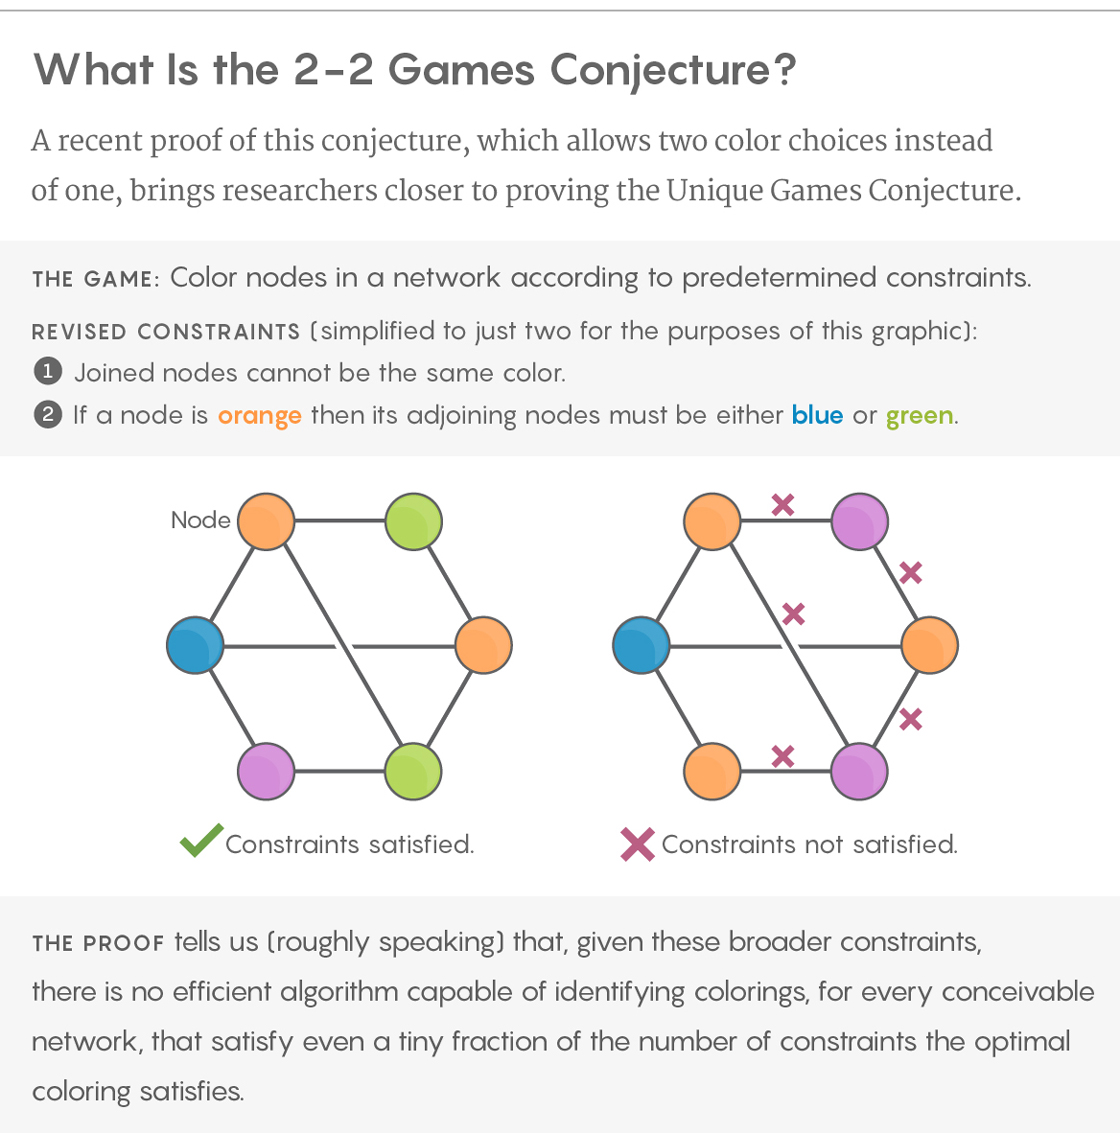
\includegraphics[width=0.7\textwidth]{images/2-2Games.jpg}
    \end{figure}{}
    
    Fonte: \cite{history}.
\end{frame}

\begin{frame}[<+->]
    \frametitle{Consequências da Prova da 2-2 Games Conjecture}
    \begin{itemize}
        \item Isso convenceu muitos céticos (alguns dos maiores céticos!) de que a UGC deve ser verdadeira, pela proximidade em relação ao 2-2 GC.
        \item É dito que isso prova \emph{metade} da UGC.
        \item Mais informações sobre a 2-2 Games Conjecture e suas consequências em \cite{history}.
    \end{itemize}
\end{frame}

\begin{frame}
  \frametitle{Exercício}
  \begin{itemize}
        \item a) Dado a instância do problema do Unique Games a seguir, construa uma instância equivalente do problema Unique Label Cover (vértices, arestas e permutações):
    
    Universo: U = \{0, 1, 2, 3\};
    
    Variáveis: $x_a, x_b, x_c, x_d$;
    
    Restrições:
    
    $f_1(x_a,x_b): f_1(0,2) = 1,f_1(1,3) = 1;$
    
    $f_2(x_a,x_c): f_2(0,2) = 1,f_2(1,3) = 1;$
    
    $f_3(x_b,x_c): f_3(0,1) = 1,f_3(2,3) = 1;$
    
    $f_4(x_c,x_d): f_4(0,3) = 1,f_4(1,2) = 1;$
    
    \item b) Verifique se todas as arestas da instância são satisfatíveis.
    
    \item c) Para essa instância pequena, é possível rapidamente verificar quantas arestas são satisfatíveis. Qual a consequência da UGC para o problema, com instâncias quaisquer?
    \end{itemize}  
\end{frame}

\begin{frame}

\bibliographystyle{abbrv}
\bibliography{ugc.bib}
\end{frame}

\end{document}
